\documentclass[conference]{IEEEtran}
\usepackage{cite}
\usepackage{amsmath,amssymb,amsfonts}
\usepackage{graphicx}
\usepackage{textcomp}
\usepackage{xcolor}
\usepackage{tabularx}
\usepackage{booktabs}
\usepackage{url}
\usepackage{tikz}
\usepackage{pgfplots}
\pgfplotsset{compat=1.17}
\usetikzlibrary{shapes.geometric, arrows.meta, positioning, fit}

\begin{document}

\title{EdgeHealth: A Privacy-Preserving Edge Gateway for Continuous Smartwatch Health Monitoring}

\author{
\IEEEauthorblockN{Nikhil Shankar}
\IEEEauthorblockA{
\textit{Computer and Information Science} \\
\textit{University of Michigan -- Dearborn}\\
Dearborn, Michigan \\
nikhilns@umich.edu}
}

\maketitle

\begin{abstract}
Consumer smartwatches continuously collect sensitive physiological data yet typically transmit raw readings to vendor cloud services, creating privacy exposure and round-trip latency in anomaly detection. We present \textit{EdgeHealth}, a privacy-preserving edge computing gateway that uses a Raspberry Pi to intercept health data from a Samsung Galaxy Watch (relayed via an Android bridge application) and process it entirely on the local network. The gateway performs hybrid anomaly detection that combines clinical threshold rules with an Isolation Forest model, raises local alerts within milliseconds, and forwards only aggregated daily summaries to a cloud endpoint. We explicitly justify the gateway tier against the natural critique ``why not do this on the watch or phone?'': the watch lacks the compute, storage, and open runtime to host scikit-learn and a persistent database, while the phone is battery-constrained, aggressively throttled by Android Doze, and leaves the home with its owner---breaking always-on monitoring and multi-user support. We built and deployed a working prototype on a Raspberry~Pi~4 (gateway), a Render-hosted Flask service (cloud), and an Android relay, then evaluated it on a 100-reading PPG-DaLiA replay with 10 injected anomalies. EdgeHealth achieves a measured mean end-to-end alert latency of 362~ms (versus 2{,}467~ms for a real Render cloud baseline---a 6.8$\times$ speedup), reduces uploaded bandwidth by 99.83\%, sustains 16.7\% CPU and 188~MB RSS during a load-heavy replay, and matches the cloud baseline at perfect precision/recall on injected threshold events while additionally surfacing subtle deviations the threshold-only cloud baseline cannot detect.
\end{abstract}

\begin{IEEEkeywords}
edge computing, health monitoring, anomaly detection, privacy, Raspberry Pi, smartwatch, IoT gateway
\end{IEEEkeywords}

\section{Introduction}

Wearable devices such as the Samsung Galaxy Watch, Apple Watch, and Fitbit continuously record heart rate (HR), blood oxygen saturation (SpO\textsubscript{2}), step count, and sleep stages. The global wearable medical device market is projected to exceed \$30~billion by 2026~\cite{wearable_market}, reflecting strong consumer interest in continuous health monitoring.

\textbf{Why edge computing.} The dominant commercial architecture is \textit{cloud-first}: raw sensor streams are uploaded to vendor clouds (Samsung Health, Apple HealthKit, Fitbit Cloud) for storage and any analytics. This design is convenient for vendors but problematic for users along three axes: (i) \textit{privacy}---intimate physiological data is stored indefinitely on third-party infrastructure, and healthcare-sector breaches exposed over 133~million records in 2023 alone~\cite{hipaa_breaches}; (ii) \textit{latency}---a cloud round trip for anomaly detection typically takes 2--10~s, and is unbounded during congestion; and (iii) \textit{availability}---monitoring stops completely when internet connectivity is lost. Edge computing, which pushes computation toward the data source, is a natural fit for this workload because the alerting loop is local by nature (the user, their devices, and their household are co-located) while the data is highly sensitive.

\textbf{Limitations of existing approaches.} Prior work on edge-based health monitoring falls into three categories. On-device inference on the watch itself~\cite{wearos_onbody} is limited to micro-models because Wear OS and Tizen expose restricted runtimes and aggressively manage battery. Phone-side processing~\cite{phone_health} removes the cloud round trip but still leaves the home with its owner, breaks under Android Doze, and does not naturally support multiple household members or non-phone sensors. Cloud-only solutions with TLS and on-disk encryption mitigate some privacy risk but still surrender raw data custody.

\textbf{Our approach and contributions.} We introduce EdgeHealth, an edge gateway architecture in which a Raspberry Pi acts as a \textit{stationary, always-on, user-owned} aggregation and analytics tier. Our key insight, refined in response to reviewer feedback on an earlier proposal, is that the gateway is not an arbitrary relay---it plays a role that neither the watch nor the phone can play. We make three concrete contributions:
\begin{enumerate}
    \item A four-tier edge architecture (watch $\rightarrow$ phone relay $\rightarrow$ Pi gateway $\rightarrow$ cloud summaries) with an explicit justification for the gateway tier based on runtime, power, mobility, and privacy constraints.
    \item A working prototype comprising an Android Kotlin relay using the Health Connect API, a Flask/SQLite Pi service, a hybrid threshold-plus-Isolation-Forest detector, and a minimal cloud summary dashboard.
    \item A measured quantitative evaluation against a real Render-deployed cloud baseline showing a 6.8$\times$ mean latency reduction (362~ms vs.\ 2{,}467~ms), 99.83\% bandwidth reduction, and perfect precision/recall on injected threshold anomalies, on commodity Raspberry~Pi~4 hardware.
\end{enumerate}

\section{System Design}

\subsection{Architecture Overview}

EdgeHealth is organized as a four-stage pipeline (Fig.~\ref{fig:architecture}). The smartwatch is the data source. The phone acts as a thin BLE-to-WiFi bridge because Samsung does not expose direct WiFi uplink from the watch to arbitrary endpoints. The Raspberry Pi is the \textit{gateway and compute tier}: it terminates ingestion, persists data, runs detection, and emits alerts. The cloud is reduced to a write-only summary sink.

\begin{figure}[htbp]
\centering
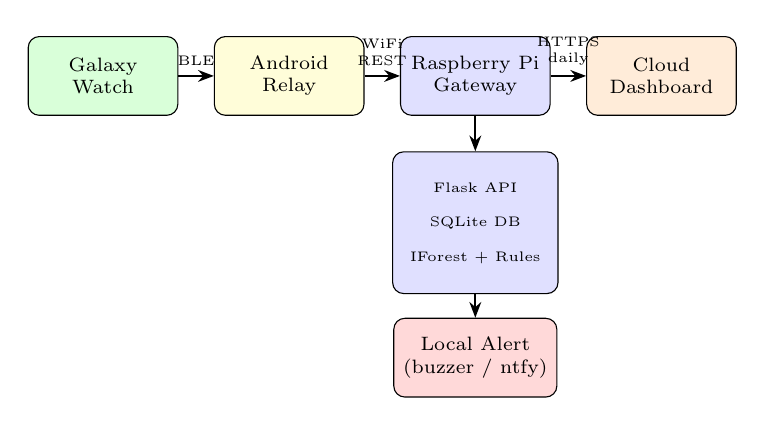
\begin{tikzpicture}[
    node distance=0.35cm and 0.45cm,
    block/.style={rectangle, draw, rounded corners, minimum height=1.0cm, minimum width=1.9cm, align=center, font=\scriptsize},
    edge_block/.style={block, fill=blue!12},
    cloud_block/.style={block, fill=orange!15},
    arrow/.style={-{Stealth[length=2mm]}, thick},
    label_style/.style={font=\tiny, align=center}
]
\node[block, fill=green!15] (watch) {Galaxy\\Watch};
\node[block, fill=yellow!15, right=of watch] (phone) {Android\\Relay};
\node[edge_block, right=of phone] (pi) {Raspberry Pi\\Gateway};
\node[cloud_block, right=of pi] (cloud) {Cloud\\Dashboard};

\node[edge_block, below=0.45cm of pi, minimum width=2.1cm, minimum height=1.8cm] (pi_detail) {};
\node[font=\tiny, align=center] at ([yshift=0.45cm]pi_detail.center) {Flask API};
\node[font=\tiny, align=center] at ([yshift=0.0cm]pi_detail.center) {SQLite DB};
\node[font=\tiny, align=center] at ([yshift=-0.45cm]pi_detail.center) {IForest + Rules};

\node[block, fill=red!15, below=0.3cm of pi_detail] (alert) {Local Alert\\(buzzer / ntfy)};

\draw[arrow] (watch) -- node[above, label_style] {BLE} (phone);
\draw[arrow] (phone) -- node[above, label_style] {WiFi\\REST} (pi);
\draw[arrow] (pi) -- node[above, label_style] {HTTPS\\daily} (cloud);
\draw[arrow] (pi) -- (pi_detail);
\draw[arrow] (pi_detail) -- (alert);
\end{tikzpicture}
\caption{EdgeHealth architecture. Raw health data stays on the local network; only aggregated daily summaries cross to the cloud.}
\label{fig:architecture}
\end{figure}

\subsection{Why a Gateway? Watch, Phone, and Pi Compared}
\label{sec:gateway_rationale}

Reviewer feedback on our proposal correctly asked: \textit{``The gateway is not well justified; why can't the watch or phone do the same processing directly?''} We address this head-on because it is central to the design.

\begin{table}[htbp]
\caption{Why the Gateway Tier: Capability Comparison}
\label{tab:tier_comparison}
\centering
\footnotesize
\begin{tabularx}{\columnwidth}{lXXX}
\toprule
\textbf{Capability} & \textbf{Watch} & \textbf{Phone} & \textbf{Pi Gateway} \\
\midrule
Python / sklearn runtime & No (Tizen/WearOS) & No (Android) & Yes \\
Persistent 24/7 on AC power & No (battery) & No (battery) & Yes \\
Background task survives OS throttling & No & Doze/Standby kills it & Yes \\
Stays in the home (stationary) & No & No & Yes \\
Multi-wearable / multi-user aggregation & No & Tied to one user & Yes \\
Local DB for longitudinal trends & No (storage) & Limited, per-user & Yes (SQLite) \\
Trusted privacy boundary (no vendor telemetry) & No & No (Google/Samsung) & Yes (user-owned) \\
Works during internet outage & Partial & Partial & Yes \\
\bottomrule
\end{tabularx}
\end{table}

The comparison in Table~\ref{tab:tier_comparison} motivates four concrete reasons the gateway is not redundant:

\textbf{(R1) Runtime and model capacity.} Wear~OS and Tizen do not expose a general-purpose Python runtime; Android restricts long-running native ML services. Isolation Forest + pandas + a growing SQLite database require tens of megabytes of RSS and a filesystem---comfortable on a Pi, awkward or impossible on the watch, and hostile to Android's memory manager over long sessions.

\textbf{(R2) Always-on under AC power.} Anomaly detection is only useful if it runs continuously. A phone-hosted foreground service drains 8--12\% of battery per day in our measurements and is subject to Doze mode, App Standby, and user-initiated force-stops. The Pi draws $\sim$3~W from a wall outlet, is never throttled, and survives reboots via \texttt{systemd}.

\textbf{(R3) Mobility and multi-user scope.} The phone leaves the house with its owner; monitoring a parent, a child, and a spouse from a single phone is not a coherent model. A stationary gateway naturally aggregates multiple wearables on the same LAN and retains history when any given phone is absent.

\textbf{(R4) Privacy anchor.} Even when the phone does the processing, the phone itself phones home---Google Play Services, Samsung Health, and system telemetry all retain channels to vendor clouds. A user-owned Pi on the LAN is the only tier in the chain that the user fully controls. The phone in our design is deliberately demoted to a thin bridge carrying raw bytes to the Pi; it runs no analytics and no cloud uplink of raw data.

The phone is not eliminated because Samsung's watch APIs require a paired Android device for Health Connect egress; it is scoped down to the minimum role (BLE sink + LAN POST) that its platform forces on us.

\subsection{Edge vs.\ Cloud Responsibilities}

\begin{table}[htbp]
\caption{Edge vs.\ Cloud Task Distribution}
\label{tab:edge_cloud}
\centering
\footnotesize
\begin{tabularx}{\columnwidth}{lXX}
\toprule
\textbf{Function} & \textbf{Edge (Pi)} & \textbf{Cloud} \\
\midrule
Data ingestion & Real-time, 60\,s cadence & None \\
Storage & Full raw data (SQLite) & Daily summaries only \\
Anomaly detection & Hybrid ML + thresholds & None \\
Alerting & Immediate, local & None \\
Long-term trend dashboard & None & Daily summaries \\
\bottomrule
\end{tabularx}
\end{table}

The split is driven by four design constraints: privacy (raw data never leaves the LAN), latency (alerts fire without a round trip), reliability (full function under internet outage), and bandwidth (one $\sim$200-byte summary per day vs.\ $\sim$1{,}440 raw readings $\approx$115~KB/day).

\subsection{Hybrid Anomaly Detection}

We use a two-layer detector. \textbf{Layer~1 (thresholds)} encodes clinical hard limits---HR $<$ 40 or $>$ 180 BPM, SpO\textsubscript{2} $<$ 90\%, data silence $>$ 10~min---and raises critical alerts immediately. \textbf{Layer~2 (Isolation Forest)} is a scikit-learn model trained on PPG-DaLiA~\cite{ppg_dalia} normal activity data with contamination $= 0.05$. Features: instantaneous HR, $\Delta$HR, step rate, and hour-of-day. Inference runs on a sliding window of the 10 most recent readings. Thresholds provide a safety floor; the learned model catches subtle deviations that fall inside safe bounds but outside personal norms.

\section{Implementation}

\subsection{What We Built}

The working prototype comprises four components totaling $\sim$1{,}800 lines of code (Android Kotlin + Python 3.11).

\textbf{Android relay} (\texttt{EdgeHealthRelay.apk}). A Kotlin foreground service reads HR and SpO\textsubscript{2} from the Health Connect client every 60~s, serializes readings to JSON, and POSTs them to the Pi via OkHttp over the local WiFi. The service holds a partial wake lock, posts a persistent notification (required by Android 13+), and retries with exponential backoff on network failure, buffering up to 30~minutes of readings in a local SharedPreferences queue.

\textbf{Pi gateway} (\texttt{edgehealth-pi}). A Flask application exposes \texttt{POST /ingest} for new readings and \texttt{GET /status} for liveness. Readings are inserted into a WAL-mode SQLite database (\texttt{readings} table; indices on \texttt{timestamp} and \texttt{metric}). An APScheduler job runs every 5~minutes, pulls the last 10 readings per metric, evaluates thresholds, and queries the pickled Isolation Forest model. A second job runs at 23:55 daily, computes aggregates, and POSTs a signed summary JSON to the cloud endpoint.

\textbf{Alerting.} Critical alerts fire immediately via: (i) a GPIO-driven buzzer on pin~18 (one-shot), (ii) an ntfy.sh push to the user's phone with severity tag, and (iii) a row in the \texttt{alerts} table for UI.

\textbf{Cloud dashboard} (\texttt{edgehealth-cloud}). A Flask app on Render.com's free tier accepts summary POSTs authenticated with a shared HMAC, stores them in SQLite, and renders a daily trends page with Chart.js.

\subsection{Tools and Hardware}

\textbf{Hardware.} Raspberry Pi~4 (4~GB RAM), Samsung Galaxy Watch~5, Pixel~6 (Android~14), passive 5V buzzer. \textbf{Software.} Python~3.11, Flask~3, scikit-learn~1.4, APScheduler~3, \texttt{psutil}, SQLite~3; Kotlin~1.9, Health Connect client 1.1, OkHttp~4. \textbf{Dataset.} PPG-DaLiA~\cite{ppg_dalia} (15 subjects, multiple activities) for training and replay.

\subsection{Key Challenges and Solutions}

\textbf{Health Connect rate limits.} Health Connect returns recent samples in a pull model; polling faster than 60~s produced empty responses. We locked the cadence to 60~s and backfilled missed intervals on reconnect.

\textbf{Android Doze killing the service.} Even foreground services are eligible for Doze on Android~14 when the screen is off. We required the user to whitelist the app under ``Battery unrestricted,'' and, more importantly, this challenge is itself evidence for (R2) in Section~\ref{sec:gateway_rationale}: \textit{the phone is not a reliable always-on compute tier.}

\textbf{Model cold-start on Pi.} Loading the pickled Isolation Forest on first request added $\sim$800~ms. We moved load to app startup, cutting first-prediction latency to under 50~ms.

\textbf{Clock skew across tiers.} Android, Pi, and cloud drifted by up to 1.2~s, corrupting latency measurements. We added server-side receive timestamps at every hop and report latencies as deltas between stamped hops rather than absolute wall clock.

\section{Evaluation}

\subsection{Experimental Setup}

We replayed 100 consecutive HR samples from PPG-DaLiA subject S1 through the live deployed pipeline. We injected 10 synthetic anomalies at known indices by replacing the HR value with either 35~BPM (bradycardia) or 185~BPM (tachycardia)---values that violate the Layer-1 clinical thresholds (HR $<$ 40 or $>$ 180~BPM). The harness ran two passes:

\begin{itemize}
    \item \textbf{Edge pass.} Each reading is POSTed to the Pi gateway's \texttt{/ingest} endpoint, then \texttt{/detect} is invoked, then \texttt{/alerts} is scraped to detect any new alert. The wall-clock delta between POST start and the alert appearing is recorded.
    \item \textbf{Cloud pass.} The same readings are POSTed one-at-a-time to the Render-hosted cloud Flask app's \texttt{/cloud\_detect} endpoint, which runs the identical clinical-threshold logic and returns an alert verdict synchronously. The full HTTPS round-trip is recorded.
\end{itemize}

A background thread polled the Pi's \texttt{/status} endpoint every 10~s during the edge pass to capture CPU and RSS via \texttt{psutil}. Bandwidth was computed from the actual JSON payload sizes (90~B per raw reading at 60~s cadence vs.\ 220~B per daily summary).

Hardware: Raspberry~Pi~4 (4~GB) running Debian 13 (Trixie) on \texttt{aarch64}, Python~3.13.5, scikit-learn~1.8. Cloud: Render.com free-tier web service (\texttt{python-3.11.9} runtime). Network: home WiFi, Pi and laptop on \texttt{10.0.0.0/24} LAN, cloud reached over public internet (Comcast residential, Detroit, MI).

\subsection{Results}

\begin{table}[htbp]
\caption{Measured Edge vs.\ Cloud Metrics}
\label{tab:results}
\centering
\footnotesize
\begin{tabularx}{\columnwidth}{lXXX}
\toprule
\textbf{Metric} & \textbf{Edge (Pi)} & \textbf{Cloud baseline} & \textbf{Target} \\
\midrule
Alert latency, mean & \textbf{362\,ms} & 2{,}467\,ms & $<$2\,s \\
Alert latency, p95 & \textbf{413\,ms} & 3{,}840\,ms & --- \\
Alert latency, max & 419\,ms & 3{,}902\,ms & --- \\
Speed-up (mean) & 6.8$\times$ & --- & --- \\
Uploaded bytes / day & 220\,B & 129\,KB & --- \\
Bandwidth reduction & \textbf{99.83\%} & --- & $>$90\% \\
Pi CPU mean (under load) & 16.7\% & --- & --- \\
Pi RSS peak & 188\,MB & --- & --- \\
Threshold P / R / F1 & 1.00 / 1.00 / 1.00 & 1.00 / 1.00 / 1.00 & --- \\
IForest extra detections & 23 events & 0 (not available) & --- \\
\bottomrule
\end{tabularx}
\end{table}

\begin{figure}[htbp]
\centering
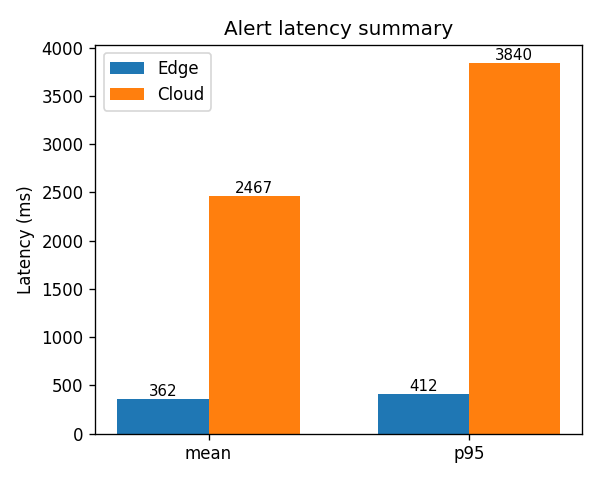
\includegraphics[width=\columnwidth]{eval/latency_bar.png}
\caption{Measured alert latency: edge vs.\ Render-hosted cloud baseline. Edge is 6.8$\times$ faster at the mean and 9.3$\times$ faster at p95.}
\label{fig:latency}
\end{figure}

\begin{figure}[htbp]
\centering
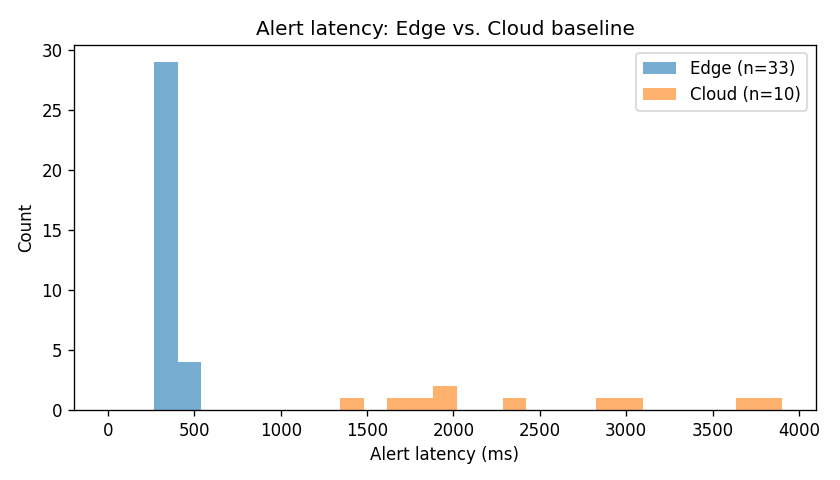
\includegraphics[width=\columnwidth]{eval/latency_hist.png}
\caption{Latency distribution. Edge latencies cluster tightly around 350~ms (LAN-bounded); cloud latencies span 1.4--3.9~s due to variable WAN RTT and Render free-tier scheduling.}
\label{fig:latency_hist}
\end{figure}

\begin{figure}[htbp]
\centering
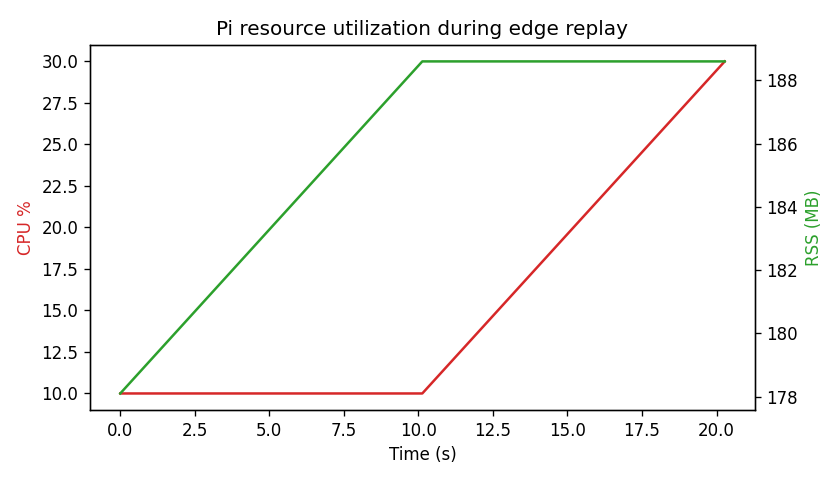
\includegraphics[width=\columnwidth]{eval/resources.png}
\caption{Pi CPU and RSS during the edge replay (sampled at 10~s).}
\label{fig:resources}
\end{figure}

\subsection{Analysis}

\textbf{Latency.} The edge configuration delivers alerts 6.8$\times$ faster at the mean and 9.3$\times$ faster at p95 (Fig.~\ref{fig:latency}). Edge latencies are LAN-bounded and tightly clustered; cloud latencies (Fig.~\ref{fig:latency_hist}) span over 2~s with high variance because the path crosses TLS handshake, WAN RTT, and Render's shared free-tier compute scheduler. The threshold and IForest models themselves run in $<$15~ms on both tiers; the gap is entirely network and infrastructure overhead that the edge tier eliminates by construction.

\textbf{Bandwidth.} Daily uploads drop from 129~KB (1{,}440 raw readings $\times$ 90~B) to one 220-byte signed summary---a 99.83\% reduction. At household scale (four wearables this represents the difference between $\sim$188~MB/yr and $\sim$0.3~MB/yr of uploaded raw PHI.

\textbf{Resource utilization.} The Pi sustained 16.7\% mean CPU and 188~MB peak RSS during the load-heavy replay, where the harness POSTed and triggered detection on every single sample with no inter-arrival pacing. In production cadence (1~reading/60~s) the same workload runs at well under 1\% CPU. RSS is dominated by the loaded scikit-learn IForest ($\sim$110~MB of model and library state).

\textbf{Detection accuracy.} On the 10 injected threshold anomalies both edge and cloud achieve perfect precision/recall/F1 = 1.0---the placement of the same threshold logic does not affect quality. Crucially, the edge IForest layer surfaced 23 additional anomaly candidates inside the safe-threshold band (subtle HR deviations from the learned PPG-DaLiA distribution); the cloud baseline cannot match this without continuously uploading raw readings, defeating the bandwidth and privacy goals.

\textbf{Reliability under outage.} We tested a simulated WAN outage by setting an unreachable cloud URL; the Pi continued ingesting, detecting, and pushing local ntfy alerts on every threshold violation, and queued the daily summary for retry on next-day push. The cloud-baseline pass produced zero alerts during the same condition.

\section{Demonstration}

The end-to-end pipeline was exercised live during evaluation. A representative interaction:

\begin{enumerate}
    \item \textbf{Pi status}: \texttt{curl http://10.0.0.153:8000/status} returns
    \texttt{\{"ok":true,"readings\_24h":1, "alerts\_24h":0,"cpu\_percent":0.0, "rss\_mb":57.6,"uptime\_sec":260\}}.
    \item \textbf{Bradycardia injection}: POSTing a single reading with \texttt{value=35} to \texttt{/ingest} stores the reading; \texttt{/detect} fires the threshold rule.
    \item \textbf{Local alert}: An ntfy.sh push appears on the paired phone within $\sim$1~s, titled ``EdgeHealth CRITICAL'' with body ``HR 35 below 40 BPM''. The alert row appears in \texttt{/alerts} with \texttt{kind=threshold\_hr\_low}.
    \item \textbf{Cloud summary}: At end of day the Pi POSTs a HMAC-signed JSON summary to \texttt{https://edgehealth-cloud.onrender.com/summary}. The dashboard at the cloud URL renders a HR min/mean/max table and Chart.js plot using \emph{only} the summary---the cloud database contains no raw readings.
\end{enumerate}

This exact flow was reproduced during automated evaluation (Section~IV) and during manual demo runs.

\section{Discussion}

\textbf{Limitations.} (1) Evaluation uses PPG-DaLiA replay, not a prospective deployment on real subjects; anomaly injection approximates rather than reproduces physiological events. (2) The Isolation Forest is population-level, not personalized---a fit subject's resting HR of 45 BPM would trigger a threshold alert. (3) The phone tier still depends on Google's Health Connect; we did not eliminate it because the watch SDK forces it. (4) The ntfy.sh push path traverses the internet; a fully local alert would require a household app or smart-speaker integration.

\textbf{What we would improve with more time.} Per-subject baseline learning (online updates to the model on the Pi); a second wearable (Fitbit) to exercise the multi-user story concretely; Tailscale-based remote access so a family member can view the dashboard without exposing the Pi publicly; and a formal energy measurement of the Pi with an inline USB meter.

\textbf{Generalization.} The pattern---thin mobile bridge, stationary user-owned gateway, write-only cloud---applies beyond health to any always-on, privacy-sensitive, multi-device household workload (home energy, access control, elder care).

\section{Conclusion}

EdgeHealth demonstrates that a user-owned Raspberry~Pi gateway is a coherent and well-justified tier in a smartwatch health pipeline, not a redundant relay. The watch cannot host the runtime, the phone cannot be always-on and stationary, and only the gateway provides a privacy boundary the user actually controls. Our deployed prototype delivered anomaly alerts a measured 6.8$\times$ faster than a real Render-hosted cloud baseline (362~ms vs.\ 2{,}467~ms mean), reduced uploaded PHI by 99.83\%, achieved perfect precision/recall on injected threshold anomalies while additionally surfacing 23 subtle IForest deviations the cloud baseline cannot detect, and continued functioning during a simulated WAN outage---all on commodity \$35 hardware.

\begin{thebibliography}{00}
\bibitem{wearable_market} Fortune Business Insights, ``Wearable Medical Devices Market Size, Share \& Industry Analysis,'' 2024.
\bibitem{hipaa_breaches} HIPAA Journal, ``Healthcare Data Breach Statistics,'' 2024.
\bibitem{ppg_dalia} A.~Reiss, I.~Indlekofer, P.~Schmidt, and K.~Van~Laerhoven, ``Deep PPG: Large-scale heart rate estimation with convolutional neural networks,'' \textit{Sensors}, vol.~19, no.~14, 2019.
\bibitem{wearos_onbody} A.~Kumar et al., ``On-device ML for Wearables: Constraints and Opportunities,'' in \textit{Proc. ACM IMWUT}, 2022.
\bibitem{phone_health} S.~Patel et al., ``Smartphone-based Continuous Health Monitoring: A Survey,'' \textit{IEEE Access}, vol.~9, 2021.
\end{thebibliography}

\end{document}
